\subsection{Preliminary results $-$ \texttt{($\alpha$, $\sigma$) $\equiv$ (8.0, 10.0)}}

% ----------------------------------- tiger1 -----------------------------------
\subsubsection{Image \texttt{tiger1}}

  \noindent\makebox[\textwidth][c]{%
  \begin{minipage}{\linewidth}
    \begin{minipage}{0.45\linewidth}
      \begin{figure}[H]
        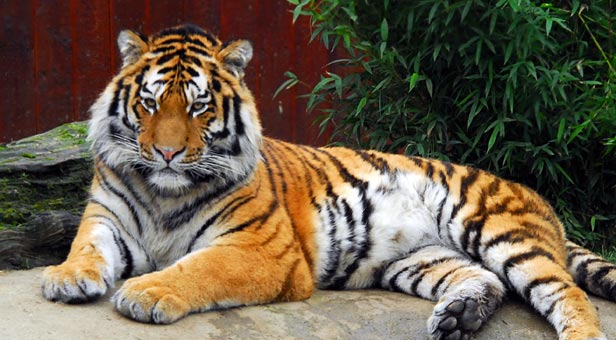
\includegraphics[scale=0.35]{../../bildat_lab3/tiger1.jpg}
        \caption{The image to be segmented into foreground and background.}
        \label{fig:04_tiger1}
      \end{figure}
    \end{minipage}
    \hfill
    \begin{minipage}{0.45\linewidth}
      \begin{figure}[H]
        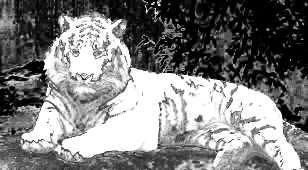
\includegraphics[scale=0.7]{./images/04/Q11/defaults/tiger1/graphcut3.png}
        \caption{Each pixel is assigned a probability proportional to the
          likelihood that it belongs to the foreground.}
        \label{fig:04_tiger1_graphcut3}
      \end{figure}
    \end{minipage}
  \end{minipage}
  }

  \noindent\makebox[\textwidth][c]{%
  \begin{minipage}{\linewidth}
    \begin{minipage}{0.45\linewidth}
      \begin{figure}[H]
        
\includegraphics[scale=0.7]{./images/04/Q11/defaults/tiger1/graphcut1.png}
        \caption{Image \ref{fig:04_tiger1_graphcut3} thresholded to $0.5$.}
        \label{fig:04_tiger1_graphcut1}
      \end{figure}
    \end{minipage}
    \hfill
    \begin{minipage}{0.45\linewidth}
      \begin{figure}[H]
        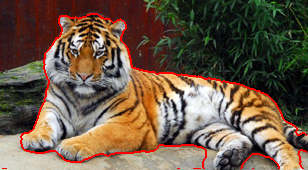
\includegraphics[scale=0.7]{./images/04/Q11/defaults/tiger1/graphcut2.png}
        \caption{The resulting of the graph cut segmetation method on image
          \texttt{tiger1}.}
        \label{fig:04_tiger1_graphcut2}
      \end{figure}
    \end{minipage}
  \end{minipage}
  }


% ----------------------------------- orange -----------------------------------
\subsubsection{Image \texttt{orange}}

  \noindent\makebox[\textwidth][c]{%
  \begin{minipage}{\linewidth}
    \begin{minipage}{0.45\linewidth}
      \begin{figure}[H]
        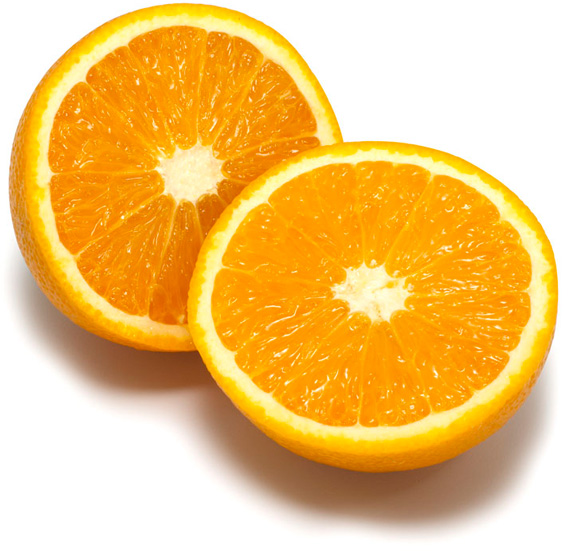
\includegraphics[scale=0.35]{../../bildat_lab3/orange.jpg}
        \caption{The image to be segmented into foreground and background.}
        \label{fig:04_orange}
      \end{figure}
    \end{minipage}
    \hfill
    \begin{minipage}{0.45\linewidth}
      \begin{figure}[H]
        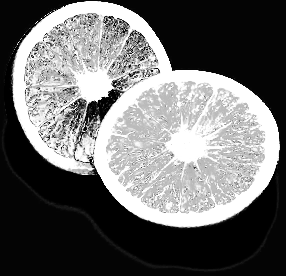
\includegraphics[scale=0.7]{./images/04/Q11/defaults/orange/graphcut3.png}
        \caption{Each pixel is assigned a probability proportional to the
          likelihood that it belongs to the foreground.}
        \label{fig:04_orange_graphcut3}
      \end{figure}
    \end{minipage}
  \end{minipage}
  }

  \noindent\makebox[\textwidth][c]{%
  \begin{minipage}{\linewidth}
    \begin{minipage}{0.45\linewidth}
      \begin{figure}[H]
        
\includegraphics[scale=0.7]{./images/04/Q11/defaults/orange/graphcut1.png}
        \caption{Image \ref{fig:04_orange_graphcut3} thresholded to $0.5$.}
        \label{fig:04_orange_graphcut1}
      \end{figure}
    \end{minipage}
    \hfill
    \begin{minipage}{0.45\linewidth}
      \begin{figure}[H]
        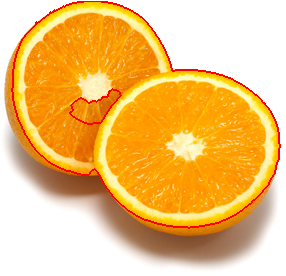
\includegraphics[scale=0.7]{./images/04/Q11/defaults/orange/graphcut2.png}
        \caption{The resulting of the graph cut segmetation method on image
          \texttt{orange}.}
        \label{fig:04_orange_graphcut2}
      \end{figure}
    \end{minipage}
  \end{minipage}
  }


% ----------------------------------- tiger2 -----------------------------------
\subsubsection{Image \texttt{tiger2}}

  \noindent\makebox[\textwidth][c]{%
  \begin{minipage}{\linewidth}
    \begin{minipage}{0.45\linewidth}
      \begin{figure}[H]
        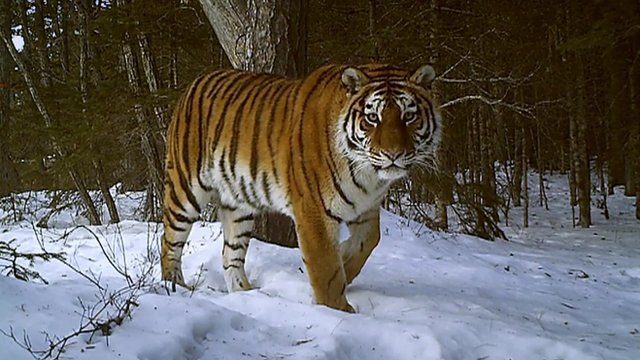
\includegraphics[scale=0.35]{../../bildat_lab3/tiger2.jpg}
        \caption{The image to be segmented into foreground and background.}
        \label{fig:04_tiger2}
      \end{figure}
    \end{minipage}
    \hfill
    \begin{minipage}{0.45\linewidth}
      \begin{figure}[H]
        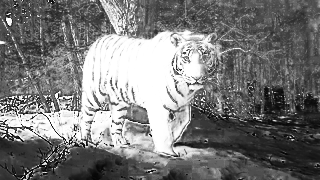
\includegraphics[scale=0.7]{./images/04/Q11/defaults/tiger2/graphcut3.png}
        \caption{Each pixel is assigned a probability proportional to the
          likelihood that it belongs to the foreground.}
        \label{fig:04_tiger2_graphcut3}
      \end{figure}
    \end{minipage}
  \end{minipage}
  }

  \noindent\makebox[\textwidth][c]{%
  \begin{minipage}{\linewidth}
    \begin{minipage}{0.45\linewidth}
      \begin{figure}[H]
        
\includegraphics[scale=0.7]{./images/04/Q11/defaults/tiger2/graphcut1.png}
        \caption{Image \ref{fig:04_tiger2_graphcut3} thresholded to $0.5$.}
        \label{fig:04_tiger2_graphcut1}
      \end{figure}
    \end{minipage}
    \hfill
    \begin{minipage}{0.45\linewidth}
      \begin{figure}[H]
        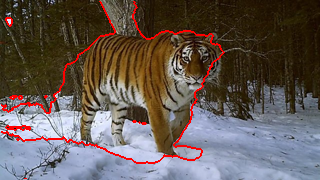
\includegraphics[scale=0.7]{./images/04/Q11/defaults/tiger2/graphcut2.png}
        \caption{The resulting of the graph cut segmetation method on image
          \texttt{tiger2}.}
        \label{fig:04_tiger2_graphcut2}
      \end{figure}
    \end{minipage}
  \end{minipage}
  }

% ----------------------------------- tiger3 -----------------------------------
\subsubsection{Image \texttt{tiger3}}

  \noindent\makebox[\textwidth][c]{%
  \begin{minipage}{\linewidth}
    \begin{minipage}{0.45\linewidth}
      \begin{figure}[H]
        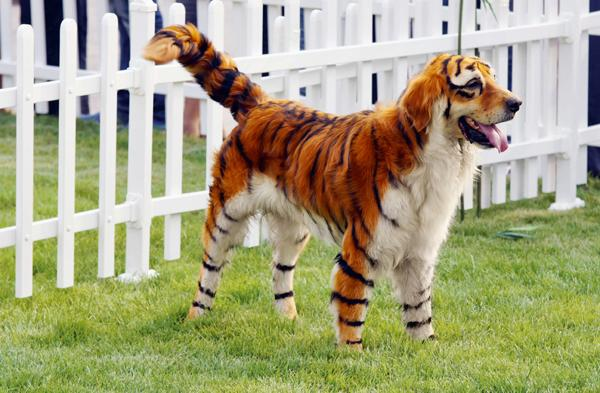
\includegraphics[scale=0.35]{../../bildat_lab3/tiger3.jpg}
        \caption{The image to be segmented into foreground and background.}
        \label{fig:04_tiger3}
      \end{figure}
    \end{minipage}
    \hfill
    \begin{minipage}{0.45\linewidth}
      \begin{figure}[H]
        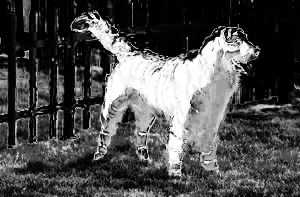
\includegraphics[scale=0.7]{./images/04/Q11/defaults/tiger3/graphcut3.png}
        \caption{Each pixel is assigned a probability proportional to the
          likelihood that it belongs to the foreground.}
        \label{fig:04_tiger3_graphcut3}
      \end{figure}
    \end{minipage}
  \end{minipage}
  }

  \noindent\makebox[\textwidth][c]{%
  \begin{minipage}{\linewidth}
    \begin{minipage}{0.45\linewidth}
      \begin{figure}[H]
        
\includegraphics[scale=0.7]{./images/04/Q11/defaults/tiger3/graphcut1.png}
        \caption{Image \ref{fig:04_tiger3_graphcut3} thresholded to $0.5$.}
        \label{fig:04_tiger3_graphcut1}
      \end{figure}
    \end{minipage}
    \hfill
    \begin{minipage}{0.45\linewidth}
      \begin{figure}[H]
        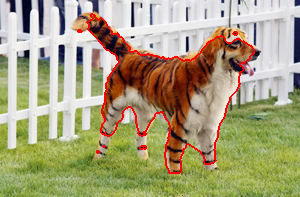
\includegraphics[scale=0.7]{./images/04/Q11/defaults/tiger3/graphcut2.png}
        \caption{The resulting of the graph cut segmetation method on image
          \texttt{tiger3}.}
        \label{fig:04_tiger3_graphcut2}
      \end{figure}
    \end{minipage}
  \end{minipage}
  }


\subsection{Varying \texttt{($\alpha$, $\sigma$)}}

% ----------------------------------- orange -----------------------------------
\subsubsection{Image \texttt{orange}}

\noindent\makebox[\textwidth][c]{%
  \begin{minipage}{0.45\linewidth}
    \begin{figure}[H]
      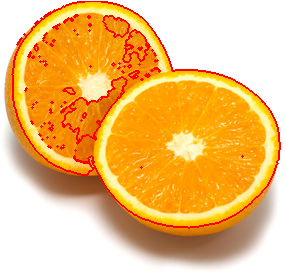
\includegraphics[scale=0.5]{./images/04/Q11/var_a_b/orange/graphcut2_a2_s4.png}
      \caption{The resulting of the graph cut segmetation method on image \texttt{orange} for
        \texttt{($\alpha$, $\sigma$)$ \equiv$ (2,4)}}
      \label{fig:04_orange2_a2_s4}
    \end{figure}
    \vfill
    \begin{figure}[H]
      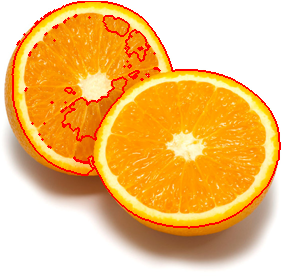
\includegraphics[scale=0.5]{./images/04/Q11/var_a_b/orange/graphcut2_a2_s6.png}
      \caption{The resulting of the graph cut segmetation method on image \texttt{orange} for
        \texttt{($\alpha$, $\sigma$)$ \equiv$ (2,6)}}
      \label{fig:04_orange2_a2_s6}
    \end{figure}
    \vfill
    \begin{figure}[H]
      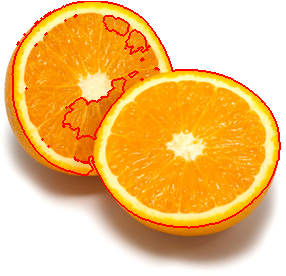
\includegraphics[scale=0.5]{./images/04/Q11/var_a_b/orange/graphcut2_a2_s10.png}
      \caption{The resulting of the graph cut segmetation method on image \texttt{orange} for
        \texttt{($\alpha$, $\sigma$)$ \equiv$ (2,10)}}
      \label{fig:04_orange2_a2_s10}
    \end{figure}
  \end{minipage}

  \begin{minipage}{0.45\linewidth}
    \begin{figure}[H]
      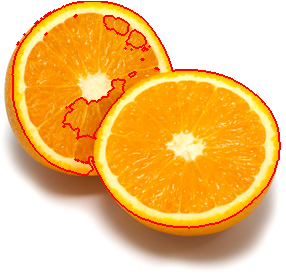
\includegraphics[scale=0.5]{./images/04/Q11/var_a_b/orange/graphcut2_a2_s12.png}
      \caption{The resulting of the graph cut segmetation method on image \texttt{orange} for
        \texttt{($\alpha$, $\sigma$)$ \equiv$ (2,12)}}
      \label{fig:04_orange2_a2_s12}
    \end{figure}
    \vfill
    \begin{figure}[H]
      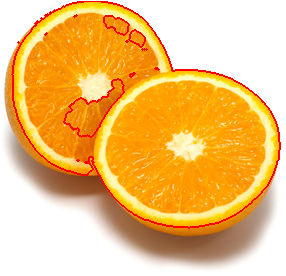
\includegraphics[scale=0.5]{./images/04/Q11/var_a_b/orange/graphcut2_a2_s16.png}
      \caption{The resulting of the graph cut segmetation method on image \texttt{orange} for
        \texttt{($\alpha$, $\sigma$)$ \equiv$ (2,16)}}
      \label{fig:04_orange2_a2_s16}
    \end{figure}
    \vfill
    \begin{figure}[H]
      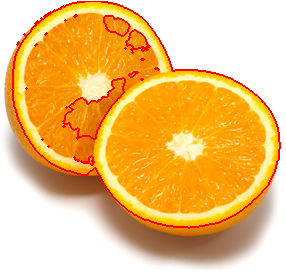
\includegraphics[scale=0.5]{./images/04/Q11/var_a_b/orange/graphcut2_a4_s4.png}
      \caption{The resulting of the graph cut segmetation method on image \texttt{orange} for
        \texttt{($\alpha$, $\sigma$)$ \equiv$ (4,4)}}
      \label{fig:04_orange2_a4_s4}
    \end{figure}
  \end{minipage}
}


\noindent\makebox[\textwidth][c]{%
  \begin{minipage}{0.45\linewidth}
    \begin{figure}[H]
      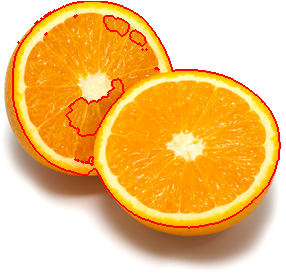
\includegraphics[scale=0.5]{./images/04/Q11/var_a_b/orange/graphcut2_a4_s6.png}
      \caption{The resulting of the graph cut segmetation method on image \texttt{orange} for
        \texttt{($\alpha$, $\sigma$)$ \equiv$ (4,6)}}
      \label{fig:04_orange2_a4_s6}
    \end{figure}
    \vfill
    \begin{figure}[H]
      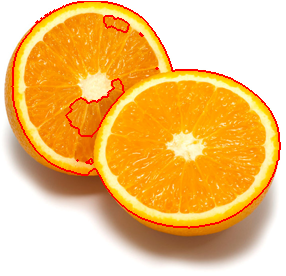
\includegraphics[scale=0.5]{./images/04/Q11/var_a_b/orange/graphcut2_a4_s10.png}
      \caption{The resulting of the graph cut segmetation method on image \texttt{orange} for
        \texttt{($\alpha$, $\sigma$)$ \equiv$ (4,10)}}
      \label{fig:04_orange2_a4_s10}
    \end{figure}
    \vfill
    \begin{figure}[H]
      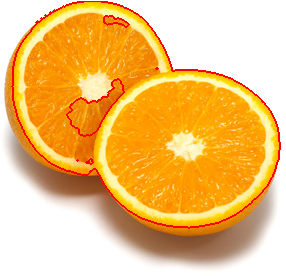
\includegraphics[scale=0.5]{./images/04/Q11/var_a_b/orange/graphcut2_a4_s12.png}
      \caption{The resulting of the graph cut segmetation method on image \texttt{orange} for
        \texttt{($\alpha$, $\sigma$)$ \equiv$ (4,12)}}
      \label{fig:04_orange2_a4_s12}
    \end{figure}
  \end{minipage}

  \begin{minipage}{0.45\linewidth}
    \begin{figure}[H]
      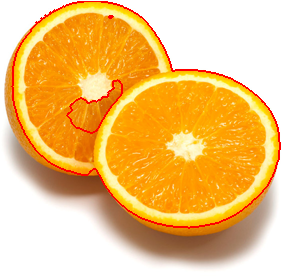
\includegraphics[scale=0.5]{./images/04/Q11/var_a_b/orange/graphcut2_a4_s16.png}
      \caption{The resulting of the graph cut segmetation method on image \texttt{orange} for
        \texttt{($\alpha$, $\sigma$)$ \equiv$ (4,16)}}
      \label{fig:04_orange2_a4_s16}
    \end{figure}
    \vfill
    \begin{figure}[H]
      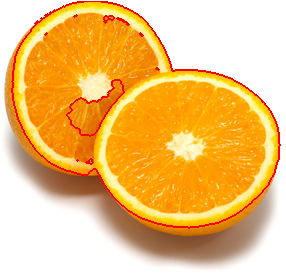
\includegraphics[scale=0.5]{./images/04/Q11/var_a_b/orange/graphcut2_a8_s4.png}
      \caption{The resulting of the graph cut segmetation method on image \texttt{orange} for
        \texttt{($\alpha$, $\sigma$)$ \equiv$ (8,4)}}
      \label{fig:04_orange2_a8_s4}
    \end{figure}
    \vfill
    \begin{figure}[H]
      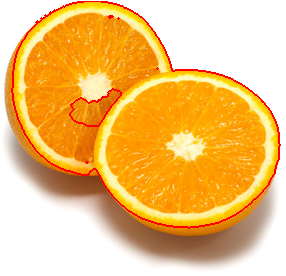
\includegraphics[scale=0.5]{./images/04/Q11/var_a_b/orange/graphcut2_a8_s6.png}
      \caption{The resulting of the graph cut segmetation method on image \texttt{orange} for
        \texttt{($\alpha$, $\sigma$)$ \equiv$ (8,6)}}
      \label{fig:04_orange2_a8_s6}
    \end{figure}
  \end{minipage}
}


\noindent\makebox[\textwidth][c]{%
  \begin{minipage}{0.45\linewidth}
    \begin{figure}[H]
      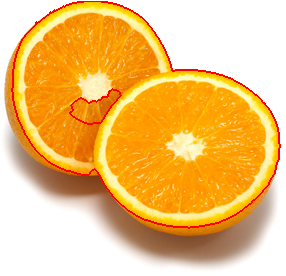
\includegraphics[scale=0.5]{./images/04/Q11/var_a_b/orange/graphcut2_a8_s10.png}
      \caption{The resulting of the graph cut segmetation method on image \texttt{orange} for
        \texttt{($\alpha$, $\sigma$)$ \equiv$ (8,10)}}
      \label{fig:04_orange2_a8_s10}
    \end{figure}
    \vfill
    \begin{figure}[H]
      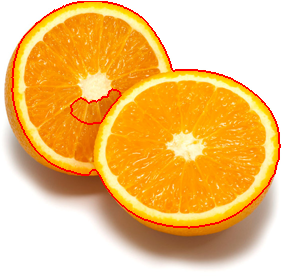
\includegraphics[scale=0.5]{./images/04/Q11/var_a_b/orange/graphcut2_a8_s12.png}
      \caption{The resulting of the graph cut segmetation method on image \texttt{orange} for
        \texttt{($\alpha$, $\sigma$)$ \equiv$ (8,12)}}
      \label{fig:04_orange2_a8_s12}
    \end{figure}
    \vfill
    \begin{figure}[H]
      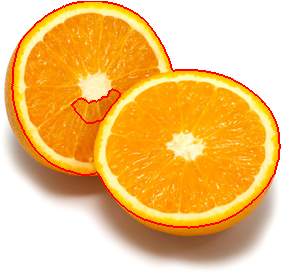
\includegraphics[scale=0.5]{./images/04/Q11/var_a_b/orange/graphcut2_a8_s16.png}
      \caption{The resulting of the graph cut segmetation method on image \texttt{orange} for
        \texttt{($\alpha$, $\sigma$)$ \equiv$ (8,16)}}
      \label{fig:04_orange2_a8_s16}
    \end{figure}
  \end{minipage}

  \begin{minipage}{0.45\linewidth}
    \begin{figure}[H]
      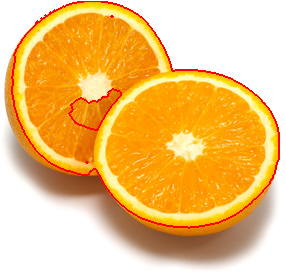
\includegraphics[scale=0.5]{./images/04/Q11/var_a_b/orange/graphcut2_a12_s4.png}
      \caption{The resulting of the graph cut segmetation method on image \texttt{orange} for
        \texttt{($\alpha$, $\sigma$)$ \equiv$ (12,4)}}
      \label{fig:04_orange2_a12_s4}
    \end{figure}
    \vfill
    \begin{figure}[H]
      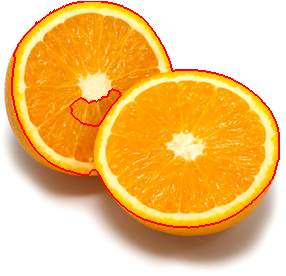
\includegraphics[scale=0.5]{./images/04/Q11/var_a_b/orange/graphcut2_a12_s6.png}
      \caption{The resulting of the graph cut segmetation method on image \texttt{orange} for
        \texttt{($\alpha$, $\sigma$)$ \equiv$ (12,6)}}
      \label{fig:04_orange2_a12_s6}
    \end{figure}
    \vfill
    \begin{figure}[H]
      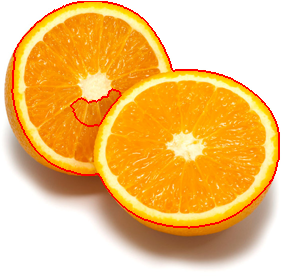
\includegraphics[scale=0.5]{./images/04/Q11/var_a_b/orange/graphcut2_a12_s10.png}
      \caption{The resulting of the graph cut segmetation method on image \texttt{orange} for
        \texttt{($\alpha$, $\sigma$)$ \equiv$ (12,10)}}
      \label{fig:04_orange2_a12_s10}
    \end{figure}
  \end{minipage}
}

\noindent\makebox[\textwidth][c]{%
  \begin{minipage}{0.45\linewidth}
    \begin{figure}[H]
      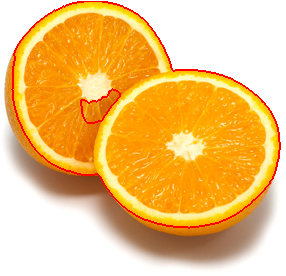
\includegraphics[scale=0.5]{./images/04/Q11/var_a_b/orange/graphcut2_a12_s12.png}
      \caption{The resulting of the graph cut segmetation method on image \texttt{orange} for
        \texttt{($\alpha$, $\sigma$)$ \equiv$ (12,12)}}
      \label{fig:04_orange2_a12_s12}
    \end{figure}
    \vfill
    \begin{figure}[H]
      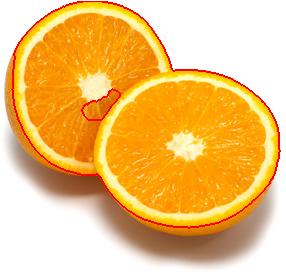
\includegraphics[scale=0.5]{./images/04/Q11/var_a_b/orange/graphcut2_a12_s16.png}
      \caption{The resulting of the graph cut segmetation method on image \texttt{orange} for
        \texttt{($\alpha$, $\sigma$)$ \equiv$ (12,16)}}
      \label{fig:04_orange2_a12_s16}
    \end{figure}
  \end{minipage}
}


% ----------------------------------- tiger1 -----------------------------------

\subsubsection{Image \texttt{tiger1}}

\noindent\makebox[\textwidth][c]{%
  \begin{minipage}{0.45\linewidth}
    \begin{figure}[H]
      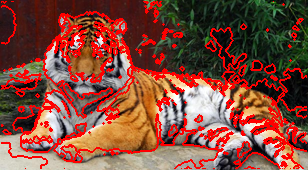
\includegraphics[scale=0.5]{./images/04/Q11/var_a_b/tiger1/graphcut2_a2_s4.png}
      \caption{The resulting of the graph cut segmetation method on image \texttt{tiger1} for
        \texttt{($\alpha$, $\sigma$)$ \equiv$ (2,4)}}
      \label{fig:04_tiger12_a2_s4}
    \end{figure}
    \vfill
    \begin{figure}[H]
      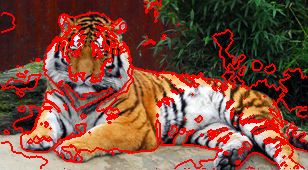
\includegraphics[scale=0.5]{./images/04/Q11/var_a_b/tiger1/graphcut2_a2_s6.png}
      \caption{The resulting of the graph cut segmetation method on image \texttt{tiger1} for
        \texttt{($\alpha$, $\sigma$)$ \equiv$ (2,6)}}
      \label{fig:04_tiger12_a2_s6}
    \end{figure}
    \vfill
    \begin{figure}[H]
      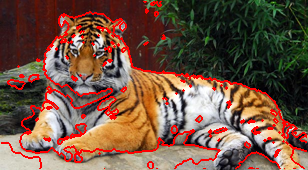
\includegraphics[scale=0.5]{./images/04/Q11/var_a_b/tiger1/graphcut2_a2_s10.png}
      \caption{The resulting of the graph cut segmetation method on image \texttt{tiger1} for
        \texttt{($\alpha$, $\sigma$)$ \equiv$ (2,10)}}
      \label{fig:04_tiger12_a2_s10}
    \end{figure}
  \end{minipage}

  \begin{minipage}{0.45\linewidth}
    \begin{figure}[H]
      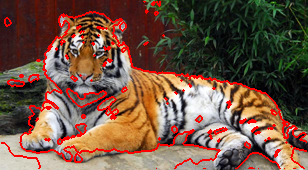
\includegraphics[scale=0.5]{./images/04/Q11/var_a_b/tiger1/graphcut2_a2_s12.png}
      \caption{The resulting of the graph cut segmetation method on image \texttt{tiger1} for
        \texttt{($\alpha$, $\sigma$)$ \equiv$ (2,12)}}
      \label{fig:04_tiger12_a2_s12}
    \end{figure}
    \vfill
    \begin{figure}[H]
      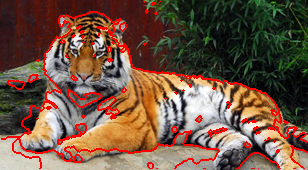
\includegraphics[scale=0.5]{./images/04/Q11/var_a_b/tiger1/graphcut2_a2_s16.png}
      \caption{The resulting of the graph cut segmetation method on image \texttt{tiger1} for
        \texttt{($\alpha$, $\sigma$)$ \equiv$ (2,16)}}
      \label{fig:04_tiger12_a2_s16}
    \end{figure}
    \vfill
    \begin{figure}[H]
      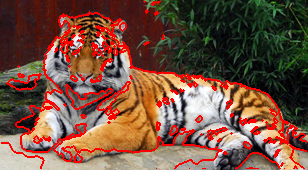
\includegraphics[scale=0.5]{./images/04/Q11/var_a_b/tiger1/graphcut2_a4_s4.png}
      \caption{The resulting of the graph cut segmetation method on image \texttt{tiger1} for
        \texttt{($\alpha$, $\sigma$)$ \equiv$ (4,4)}}
      \label{fig:04_tiger12_a4_s4}
    \end{figure}
  \end{minipage}
}


\noindent\makebox[\textwidth][c]{%
  \begin{minipage}{0.45\linewidth}
    \begin{figure}[H]
      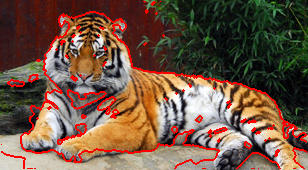
\includegraphics[scale=0.5]{./images/04/Q11/var_a_b/tiger1/graphcut2_a4_s6.png}
      \caption{The resulting of the graph cut segmetation method on image \texttt{tiger1} for
        \texttt{($\alpha$, $\sigma$)$ \equiv$ (4,6)}}
      \label{fig:04_tiger12_a4_s6}
    \end{figure}
    \vfill
    \begin{figure}[H]
      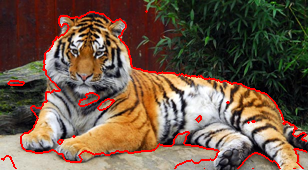
\includegraphics[scale=0.5]{./images/04/Q11/var_a_b/tiger1/graphcut2_a4_s10.png}
      \caption{The resulting of the graph cut segmetation method on image \texttt{tiger1} for
        \texttt{($\alpha$, $\sigma$)$ \equiv$ (4,10)}}
      \label{fig:04_tiger12_a4_s10}
    \end{figure}
    \vfill
    \begin{figure}[H]
      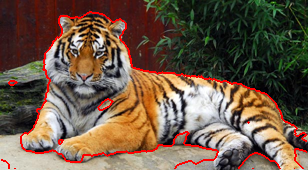
\includegraphics[scale=0.5]{./images/04/Q11/var_a_b/tiger1/graphcut2_a4_s12.png}
      \caption{The resulting of the graph cut segmetation method on image \texttt{tiger1} for
        \texttt{($\alpha$, $\sigma$)$ \equiv$ (4,12)}}
      \label{fig:04_tiger12_a4_s12}
    \end{figure}
  \end{minipage}

  \begin{minipage}{0.45\linewidth}
    \begin{figure}[H]
      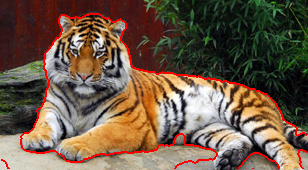
\includegraphics[scale=0.5]{./images/04/Q11/var_a_b/tiger1/graphcut2_a4_s16.png}
      \caption{The resulting of the graph cut segmetation method on image \texttt{tiger1} for
        \texttt{($\alpha$, $\sigma$)$ \equiv$ (4,16)}}
      \label{fig:04_tiger12_a4_s16}
    \end{figure}
    \vfill
    \begin{figure}[H]
      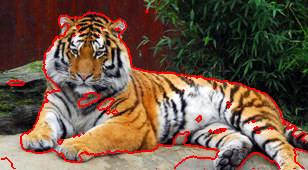
\includegraphics[scale=0.5]{./images/04/Q11/var_a_b/tiger1/graphcut2_a8_s4.png}
      \caption{The resulting of the graph cut segmetation method on image \texttt{tiger1} for
        \texttt{($\alpha$, $\sigma$)$ \equiv$ (8,4)}}
      \label{fig:04_tiger12_a8_s4}
    \end{figure}
    \vfill
    \begin{figure}[H]
      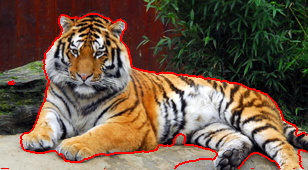
\includegraphics[scale=0.5]{./images/04/Q11/var_a_b/tiger1/graphcut2_a8_s6.png}
      \caption{The resulting of the graph cut segmetation method on image \texttt{tiger1} for
        \texttt{($\alpha$, $\sigma$)$ \equiv$ (8,6)}}
      \label{fig:04_tiger12_a8_s6}
    \end{figure}
  \end{minipage}
}


\noindent\makebox[\textwidth][c]{%
  \begin{minipage}{0.45\linewidth}
    \begin{figure}[H]
      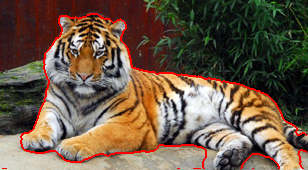
\includegraphics[scale=0.5]{./images/04/Q11/var_a_b/tiger1/graphcut2_a8_s10.png}
      \caption{The resulting of the graph cut segmetation method on image \texttt{tiger1} for
        \texttt{($\alpha$, $\sigma$)$ \equiv$ (8,10)}}
      \label{fig:04_tiger12_a8_s10}
    \end{figure}
    \vfill
    \begin{figure}[H]
      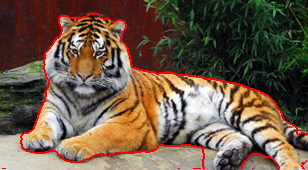
\includegraphics[scale=0.5]{./images/04/Q11/var_a_b/tiger1/graphcut2_a8_s12.png}
      \caption{The resulting of the graph cut segmetation method on image \texttt{tiger1} for
        \texttt{($\alpha$, $\sigma$)$ \equiv$ (8,12)}}
      \label{fig:04_tiger12_a8_s12}
    \end{figure}
    \vfill
    \begin{figure}[H]
      \includegraphics[scale=0.5]{./images/04/Q11/var_a_b/tiger1/graphcut2_a8_s16.png}
      \caption{The resulting of the graph cut segmetation method on image \texttt{tiger1} for
        \texttt{($\alpha$, $\sigma$)$ \equiv$ (8,16)}}
      \label{fig:04_tiger12_a8_s16}
    \end{figure}
  \end{minipage}

  \begin{minipage}{0.45\linewidth}
    \begin{figure}[H]
      \includegraphics[scale=0.5]{./images/04/Q11/var_a_b/tiger1/graphcut2_a12_s4.png}
      \caption{The resulting of the graph cut segmetation method on image \texttt{tiger1} for
        \texttt{($\alpha$, $\sigma$)$ \equiv$ (12,4)}}
      \label{fig:04_tiger12_a12_s4}
    \end{figure}
    \vfill
    \begin{figure}[H]
      \includegraphics[scale=0.5]{./images/04/Q11/var_a_b/tiger1/graphcut2_a12_s6.png}
      \caption{The resulting of the graph cut segmetation method on image \texttt{tiger1} for
        \texttt{($\alpha$, $\sigma$)$ \equiv$ (12,6)}}
      \label{fig:04_tiger12_a12_s6}
    \end{figure}
    \vfill
    \begin{figure}[H]
      \includegraphics[scale=0.5]{./images/04/Q11/var_a_b/tiger1/graphcut2_a12_s10.png}
      \caption{The resulting of the graph cut segmetation method on image \texttt{tiger1} for
        \texttt{($\alpha$, $\sigma$)$ \equiv$ (12,10)}}
      \label{fig:04_tiger12_a12_s10}
    \end{figure}
  \end{minipage}
}

\noindent\makebox[\textwidth][c]{%
  \begin{minipage}{0.45\linewidth}
    \begin{figure}[H]
      \includegraphics[scale=0.5]{./images/04/Q11/var_a_b/tiger1/graphcut2_a12_s12.png}
      \caption{The resulting of the graph cut segmetation method on image \texttt{tiger1} for
        \texttt{($\alpha$, $\sigma$)$ \equiv$ (12,12)}}
      \label{fig:04_tiger12_a12_s12}
    \end{figure}
    \vfill
    \begin{figure}[H]
      \includegraphics[scale=0.5]{./images/04/Q11/var_a_b/tiger1/graphcut2_a12_s16.png}
      \caption{The resulting of the graph cut segmetation method on image \texttt{tiger1} for
        \texttt{($\alpha$, $\sigma$)$ \equiv$ (12,16)}}
      \label{fig:04_tiger12_a12_s16}
    \end{figure}
  \end{minipage}
}



% ----------------------------------- tiger2 -----------------------------------

\subsubsection{Image \texttt{tiger2}}

\noindent\makebox[\textwidth][c]{%
  \begin{minipage}{0.45\linewidth}
    \begin{figure}[H]
      \includegraphics[scale=0.5]{./images/04/Q11/var_a_b/tiger2/graphcut2_a2_s4.png}
      \caption{The resulting of the graph cut segmetation method on image \texttt{tiger2} for
        \texttt{($\alpha$, $\sigma$)$ \equiv$ (2,4)}}
      \label{fig:04_tiger22_a2_s4}
    \end{figure}
    \vfill
    \begin{figure}[H]
      \includegraphics[scale=0.5]{./images/04/Q11/var_a_b/tiger2/graphcut2_a2_s6.png}
      \caption{The resulting of the graph cut segmetation method on image \texttt{tiger2} for
        \texttt{($\alpha$, $\sigma$)$ \equiv$ (2,6)}}
      \label{fig:04_tiger22_a2_s6}
    \end{figure}
    \vfill
    \begin{figure}[H]
      \includegraphics[scale=0.5]{./images/04/Q11/var_a_b/tiger2/graphcut2_a2_s10.png}
      \caption{The resulting of the graph cut segmetation method on image \texttt{tiger2} for
        \texttt{($\alpha$, $\sigma$)$ \equiv$ (2,10)}}
      \label{fig:04_tiger22_a2_s10}
    \end{figure}
  \end{minipage}

  \begin{minipage}{0.45\linewidth}
    \begin{figure}[H]
      \includegraphics[scale=0.5]{./images/04/Q11/var_a_b/tiger2/graphcut2_a2_s12.png}
      \caption{The resulting of the graph cut segmetation method on image \texttt{tiger2} for
        \texttt{($\alpha$, $\sigma$)$ \equiv$ (2,12)}}
      \label{fig:04_tiger22_a2_s12}
    \end{figure}
    \vfill
    \begin{figure}[H]
      \includegraphics[scale=0.5]{./images/04/Q11/var_a_b/tiger2/graphcut2_a2_s16.png}
      \caption{The resulting of the graph cut segmetation method on image \texttt{tiger2} for
        \texttt{($\alpha$, $\sigma$)$ \equiv$ (2,16)}}
      \label{fig:04_tiger22_a2_s16}
    \end{figure}
    \vfill
    \begin{figure}[H]
      \includegraphics[scale=0.5]{./images/04/Q11/var_a_b/tiger2/graphcut2_a4_s4.png}
      \caption{The resulting of the graph cut segmetation method on image \texttt{tiger2} for
        \texttt{($\alpha$, $\sigma$)$ \equiv$ (4,4)}}
      \label{fig:04_tiger22_a4_s4}
    \end{figure}
  \end{minipage}
}


\noindent\makebox[\textwidth][c]{%
  \begin{minipage}{0.45\linewidth}
    \begin{figure}[H]
      \includegraphics[scale=0.5]{./images/04/Q11/var_a_b/tiger2/graphcut2_a4_s6.png}
      \caption{The resulting of the graph cut segmetation method on image \texttt{tiger2} for
        \texttt{($\alpha$, $\sigma$)$ \equiv$ (4,6)}}
      \label{fig:04_tiger22_a4_s6}
    \end{figure}
    \vfill
    \begin{figure}[H]
      \includegraphics[scale=0.5]{./images/04/Q11/var_a_b/tiger2/graphcut2_a4_s10.png}
      \caption{The resulting of the graph cut segmetation method on image \texttt{tiger2} for
        \texttt{($\alpha$, $\sigma$)$ \equiv$ (4,10)}}
      \label{fig:04_tiger22_a4_s10}
    \end{figure}
    \vfill
    \begin{figure}[H]
      \includegraphics[scale=0.5]{./images/04/Q11/var_a_b/tiger2/graphcut2_a4_s12.png}
      \caption{The resulting of the graph cut segmetation method on image \texttt{tiger2} for
        \texttt{($\alpha$, $\sigma$)$ \equiv$ (4,12)}}
      \label{fig:04_tiger22_a4_s12}
    \end{figure}
  \end{minipage}

  \begin{minipage}{0.45\linewidth}
    \begin{figure}[H]
      \includegraphics[scale=0.5]{./images/04/Q11/var_a_b/tiger2/graphcut2_a4_s16.png}
      \caption{The resulting of the graph cut segmetation method on image \texttt{tiger2} for
        \texttt{($\alpha$, $\sigma$)$ \equiv$ (4,16)}}
      \label{fig:04_tiger22_a4_s16}
    \end{figure}
    \vfill
    \begin{figure}[H]
      \includegraphics[scale=0.5]{./images/04/Q11/var_a_b/tiger2/graphcut2_a8_s4.png}
      \caption{The resulting of the graph cut segmetation method on image \texttt{tiger2} for
        \texttt{($\alpha$, $\sigma$)$ \equiv$ (8,4)}}
      \label{fig:04_tiger22_a8_s4}
    \end{figure}
    \vfill
    \begin{figure}[H]
      \includegraphics[scale=0.5]{./images/04/Q11/var_a_b/tiger2/graphcut2_a8_s6.png}
      \caption{The resulting of the graph cut segmetation method on image \texttt{tiger2} for
        \texttt{($\alpha$, $\sigma$)$ \equiv$ (8,6)}}
      \label{fig:04_tiger22_a8_s6}
    \end{figure}
  \end{minipage}
}


\noindent\makebox[\textwidth][c]{%
  \begin{minipage}{0.45\linewidth}
    \begin{figure}[H]
      \includegraphics[scale=0.5]{./images/04/Q11/var_a_b/tiger2/graphcut2_a8_s10.png}
      \caption{The resulting of the graph cut segmetation method on image \texttt{tiger2} for
        \texttt{($\alpha$, $\sigma$)$ \equiv$ (8,10)}}
      \label{fig:04_tiger22_a8_s10}
    \end{figure}
    \vfill
    \begin{figure}[H]
      \includegraphics[scale=0.5]{./images/04/Q11/var_a_b/tiger2/graphcut2_a8_s12.png}
      \caption{The resulting of the graph cut segmetation method on image \texttt{tiger2} for
        \texttt{($\alpha$, $\sigma$)$ \equiv$ (8,12)}}
      \label{fig:04_tiger22_a8_s12}
    \end{figure}
    \vfill
    \begin{figure}[H]
      \includegraphics[scale=0.5]{./images/04/Q11/var_a_b/tiger2/graphcut2_a8_s16.png}
      \caption{The resulting of the graph cut segmetation method on image \texttt{tiger2} for
        \texttt{($\alpha$, $\sigma$)$ \equiv$ (8,16)}}
      \label{fig:04_tiger22_a8_s16}
    \end{figure}
  \end{minipage}

  \begin{minipage}{0.45\linewidth}
    \begin{figure}[H]
      \includegraphics[scale=0.5]{./images/04/Q11/var_a_b/tiger2/graphcut2_a12_s4.png}
      \caption{The resulting of the graph cut segmetation method on image \texttt{tiger2} for
        \texttt{($\alpha$, $\sigma$)$ \equiv$ (12,4)}}
      \label{fig:04_tiger22_a12_s4}
    \end{figure}
    \vfill
    \begin{figure}[H]
      \includegraphics[scale=0.5]{./images/04/Q11/var_a_b/tiger2/graphcut2_a12_s6.png}
      \caption{The resulting of the graph cut segmetation method on image \texttt{tiger2} for
        \texttt{($\alpha$, $\sigma$)$ \equiv$ (12,6)}}
      \label{fig:04_tiger22_a12_s6}
    \end{figure}
    \vfill
    \begin{figure}[H]
      \includegraphics[scale=0.5]{./images/04/Q11/var_a_b/tiger2/graphcut2_a12_s10.png}
      \caption{The resulting of the graph cut segmetation method on image \texttt{tiger2} for
        \texttt{($\alpha$, $\sigma$)$ \equiv$ (12,10)}}
      \label{fig:04_tiger22_a12_s10}
    \end{figure}
  \end{minipage}
}

\noindent\makebox[\textwidth][c]{%
  \begin{minipage}{0.45\linewidth}
    \begin{figure}[H]
      \includegraphics[scale=0.5]{./images/04/Q11/var_a_b/tiger2/graphcut2_a12_s12.png}
      \caption{The resulting of the graph cut segmetation method on image \texttt{tiger2} for
        \texttt{($\alpha$, $\sigma$)$ \equiv$ (12,12)}}
      \label{fig:04_tiger22_a12_s12}
    \end{figure}
    \vfill
    \begin{figure}[H]
      \includegraphics[scale=0.5]{./images/04/Q11/var_a_b/tiger2/graphcut2_a12_s16.png}
      \caption{The resulting of the graph cut segmetation method on image \texttt{tiger2} for
        \texttt{($\alpha$, $\sigma$)$ \equiv$ (12,16)}}
      \label{fig:04_tiger22_a12_s16}
    \end{figure}
  \end{minipage}
}



% ----------------------------------- tiger3 -----------------------------------

\subsubsection{Image \texttt{tiger3}}

\noindent\makebox[\textwidth][c]{%
  \begin{minipage}{0.45\linewidth}
    \begin{figure}[H]
      \includegraphics[scale=0.5]{./images/04/Q11/var_a_b/tiger3/graphcut2_a2_s4.png}
      \caption{The resulting of the graph cut segmetation method on image \texttt{tiger3} for
        \texttt{($\alpha$, $\sigma$)$ \equiv$ (2,4)}}
      \label{fig:04_tiger32_a2_s4}
    \end{figure}
    \vfill
    \begin{figure}[H]
      \includegraphics[scale=0.5]{./images/04/Q11/var_a_b/tiger3/graphcut2_a2_s6.png}
      \caption{The resulting of the graph cut segmetation method on image \texttt{tiger3} for
        \texttt{($\alpha$, $\sigma$)$ \equiv$ (2,6)}}
      \label{fig:04_tiger32_a2_s6}
    \end{figure}
    \vfill
    \begin{figure}[H]
      \includegraphics[scale=0.5]{./images/04/Q11/var_a_b/tiger3/graphcut2_a2_s10.png}
      \caption{The resulting of the graph cut segmetation method on image \texttt{tiger3} for
        \texttt{($\alpha$, $\sigma$)$ \equiv$ (2,10)}}
      \label{fig:04_tiger32_a2_s10}
    \end{figure}
  \end{minipage}

  \begin{minipage}{0.45\linewidth}
    \begin{figure}[H]
      \includegraphics[scale=0.5]{./images/04/Q11/var_a_b/tiger3/graphcut2_a2_s12.png}
      \caption{The resulting of the graph cut segmetation method on image \texttt{tiger3} for
        \texttt{($\alpha$, $\sigma$)$ \equiv$ (2,12)}}
      \label{fig:04_tiger32_a2_s12}
    \end{figure}
    \vfill
    \begin{figure}[H]
      \includegraphics[scale=0.5]{./images/04/Q11/var_a_b/tiger3/graphcut2_a2_s16.png}
      \caption{The resulting of the graph cut segmetation method on image \texttt{tiger3} for
        \texttt{($\alpha$, $\sigma$)$ \equiv$ (2,16)}}
      \label{fig:04_tiger32_a2_s16}
    \end{figure}
    \vfill
    \begin{figure}[H]
      \includegraphics[scale=0.5]{./images/04/Q11/var_a_b/tiger3/graphcut2_a4_s4.png}
      \caption{The resulting of the graph cut segmetation method on image \texttt{tiger3} for
        \texttt{($\alpha$, $\sigma$)$ \equiv$ (4,4)}}
      \label{fig:04_tiger32_a4_s4}
    \end{figure}
  \end{minipage}
}


\noindent\makebox[\textwidth][c]{%
  \begin{minipage}{0.45\linewidth}
    \begin{figure}[H]
      \includegraphics[scale=0.5]{./images/04/Q11/var_a_b/tiger3/graphcut2_a4_s6.png}
      \caption{The resulting of the graph cut segmetation method on image \texttt{tiger3} for
        \texttt{($\alpha$, $\sigma$)$ \equiv$ (4,6)}}
      \label{fig:04_tiger32_a4_s6}
    \end{figure}
    \vfill
    \begin{figure}[H]
      \includegraphics[scale=0.5]{./images/04/Q11/var_a_b/tiger3/graphcut2_a4_s10.png}
      \caption{The resulting of the graph cut segmetation method on image \texttt{tiger3} for
        \texttt{($\alpha$, $\sigma$)$ \equiv$ (4,10)}}
      \label{fig:04_tiger32_a4_s10}
    \end{figure}
    \vfill
    \begin{figure}[H]
      \includegraphics[scale=0.5]{./images/04/Q11/var_a_b/tiger3/graphcut2_a4_s12.png}
      \caption{The resulting of the graph cut segmetation method on image \texttt{tiger3} for
        \texttt{($\alpha$, $\sigma$)$ \equiv$ (4,12)}}
      \label{fig:04_tiger32_a4_s12}
    \end{figure}
  \end{minipage}

  \begin{minipage}{0.45\linewidth}
    \begin{figure}[H]
      \includegraphics[scale=0.5]{./images/04/Q11/var_a_b/tiger3/graphcut2_a4_s16.png}
      \caption{The resulting of the graph cut segmetation method on image \texttt{tiger3} for
        \texttt{($\alpha$, $\sigma$)$ \equiv$ (4,16)}}
      \label{fig:04_tiger32_a4_s16}
    \end{figure}
    \vfill
    \begin{figure}[H]
      \includegraphics[scale=0.5]{./images/04/Q11/var_a_b/tiger3/graphcut2_a8_s4.png}
      \caption{The resulting of the graph cut segmetation method on image \texttt{tiger3} for
        \texttt{($\alpha$, $\sigma$)$ \equiv$ (8,4)}}
      \label{fig:04_tiger32_a8_s4}
    \end{figure}
    \vfill
    \begin{figure}[H]
      \includegraphics[scale=0.5]{./images/04/Q11/var_a_b/tiger3/graphcut2_a8_s6.png}
      \caption{The resulting of the graph cut segmetation method on image \texttt{tiger3} for
        \texttt{($\alpha$, $\sigma$)$ \equiv$ (8,6)}}
      \label{fig:04_tiger32_a8_s6}
    \end{figure}
  \end{minipage}
}


\noindent\makebox[\textwidth][c]{%
  \begin{minipage}{0.45\linewidth}
    \begin{figure}[H]
      \includegraphics[scale=0.5]{./images/04/Q11/var_a_b/tiger3/graphcut2_a8_s10.png}
      \caption{The resulting of the graph cut segmetation method on image \texttt{tiger3} for
        \texttt{($\alpha$, $\sigma$)$ \equiv$ (8,10)}}
      \label{fig:04_tiger32_a8_s10}
    \end{figure}
    \vfill
    \begin{figure}[H]
      \includegraphics[scale=0.5]{./images/04/Q11/var_a_b/tiger3/graphcut2_a8_s12.png}
      \caption{The resulting of the graph cut segmetation method on image \texttt{tiger3} for
        \texttt{($\alpha$, $\sigma$)$ \equiv$ (8,12)}}
      \label{fig:04_tiger32_a8_s12}
    \end{figure}
    \vfill
    \begin{figure}[H]
      \includegraphics[scale=0.5]{./images/04/Q11/var_a_b/tiger3/graphcut2_a8_s16.png}
      \caption{The resulting of the graph cut segmetation method on image \texttt{tiger3} for
        \texttt{($\alpha$, $\sigma$)$ \equiv$ (8,16)}}
      \label{fig:04_tiger32_a8_s16}
    \end{figure}
  \end{minipage}

  \begin{minipage}{0.45\linewidth}
    \begin{figure}[H]
      \includegraphics[scale=0.5]{./images/04/Q11/var_a_b/tiger3/graphcut2_a12_s4.png}
      \caption{The resulting of the graph cut segmetation method on image \texttt{tiger3} for
        \texttt{($\alpha$, $\sigma$)$ \equiv$ (12,4)}}
      \label{fig:04_tiger32_a12_s4}
    \end{figure}
    \vfill
    \begin{figure}[H]
      \includegraphics[scale=0.5]{./images/04/Q11/var_a_b/tiger3/graphcut2_a12_s6.png}
      \caption{The resulting of the graph cut segmetation method on image \texttt{tiger3} for
        \texttt{($\alpha$, $\sigma$)$ \equiv$ (12,6)}}
      \label{fig:04_tiger32_a12_s6}
    \end{figure}
    \vfill
    \begin{figure}[H]
      \includegraphics[scale=0.5]{./images/04/Q11/var_a_b/tiger3/graphcut2_a12_s10.png}
      \caption{The resulting of the graph cut segmetation method on image \texttt{tiger3} for
        \texttt{($\alpha$, $\sigma$)$ \equiv$ (12,10)}}
      \label{fig:04_tiger32_a12_s10}
    \end{figure}
  \end{minipage}
}

\noindent\makebox[\textwidth][c]{%
  \begin{minipage}{0.45\linewidth}
    \begin{figure}[H]
      \includegraphics[scale=0.5]{./images/04/Q11/var_a_b/tiger3/graphcut2_a12_s12.png}
      \caption{The resulting of the graph cut segmetation method on image \texttt{tiger3} for
        \texttt{($\alpha$, $\sigma$)$ \equiv$ (12,12)}}
      \label{fig:04_tiger32_a12_s12}
    \end{figure}
    \vfill
    \begin{figure}[H]
      \includegraphics[scale=0.5]{./images/04/Q11/var_a_b/tiger3/graphcut2_a12_s16.png}
      \caption{The resulting of the graph cut segmetation method on image \texttt{tiger3} for
        \texttt{($\alpha$, $\sigma$)$ \equiv$ (12,16)}}
      \label{fig:04_tiger32_a12_s16}
    \end{figure}
  \end{minipage}
}


\subsection{Question 11}

Images \ref{fig:04_orange2_a2_s4} - \ref{fig:04_tiger32_a12_s16} illustrate
the resulting segmentation of images \texttt{orange, tiger\{1,2,3\}} for
all combinations of \texttt{$\alpha = [2.0, 4.0, 8.0, 12.0]$} and
\texttt{$\sigma = [4.0, 6.0, 10.0, 12.0, 16.0]$}.

From these images we can deduce that the optimal setting for variables
\texttt{$\alpha, \sigma$} is in the vicinity of $(8.0, 10.0)$. For a higher
values the resulting segmentation remains almost the same, although it becomes
coarse. The opposite can be said for smaller values of \texttt{$\alpha, \sigma$}:
the lower their values, the more sensitive and less accurate becomes the
division between the foreground and background pixels.


\subsection{Question 12}

Figures \ref{fig:04_tiger1_K_16} - \ref{fig:04_tiger1_K_1} illustrate the
resulting segmentation of image \texttt{tiger1} for values of
\texttt{K $\in$ [1, 16], K $\in \mathbb{Z}$}.

As is evident from these images, the minimum value for \texttt{K} that can still
produce reasonably accurate segmentation results for image \texttt{tiger1} is
\texttt{K=6}.


\noindent\makebox[\textwidth][c]{%
\begin{minipage}{\linewidth}
  \begin{minipage}{0.45\linewidth}
    \begin{figure}[H]
      \includegraphics[scale=0.8]{./images/04/Q12/graphcut2_k_16}
      \caption{Image \texttt{tiger1} segmented with \texttt{K = 16}}
      \label{fig:04_tiger1_K_16}
    \end{figure}
  \end{minipage}
  \hfill
  \begin{minipage}{0.45\linewidth}
    \begin{figure}[H]
      \includegraphics[scale=0.8]{./images/04/Q12/graphcut2_k_15}
      \caption{Image \texttt{tiger1} segmented with \texttt{K = 15}}
      \label{fig:04_tiger1_K_15}
    \end{figure}
  \end{minipage}
\end{minipage}
}

\noindent\makebox[\textwidth][c]{%
\begin{minipage}{\linewidth}
  \begin{minipage}{0.45\linewidth}
    \begin{figure}[H]
      \includegraphics[scale=0.8]{./images/04/Q12/graphcut2_k_14}
      \caption{Image \texttt{tiger1} segmented with \texttt{K = 14}}
      \label{fig:04_tiger1_K_14}
    \end{figure}
  \end{minipage}
  \hfill
  \begin{minipage}{0.45\linewidth}
    \begin{figure}[H]
      \includegraphics[scale=0.8]{./images/04/Q12/graphcut2_k_13}
      \caption{Image \texttt{tiger1} segmented with \texttt{K = 13}}
      \label{fig:04_tiger1_K_13}
    \end{figure}
  \end{minipage}
\end{minipage}
}

\noindent\makebox[\textwidth][c]{%
\begin{minipage}{\linewidth}
  \begin{minipage}{0.45\linewidth}
    \begin{figure}[H]
      \includegraphics[scale=0.8]{./images/04/Q12/graphcut2_k_12}
      \caption{Image \texttt{tiger1} segmented with \texttt{K = 12}}
      \label{fig:04_tiger1_K_12}
    \end{figure}
  \end{minipage}
  \hfill
  \begin{minipage}{0.45\linewidth}
    \begin{figure}[H]
      \includegraphics[scale=0.8]{./images/04/Q12/graphcut2_k_11}
      \caption{Image \texttt{tiger1} segmented with \texttt{K = 11}}
      \label{fig:04_tiger1_K_11}
    \end{figure}
  \end{minipage}
\end{minipage}
}

\noindent\makebox[\textwidth][c]{%
\begin{minipage}{\linewidth}
  \begin{minipage}{0.45\linewidth}
    \begin{figure}[H]
      \includegraphics[scale=0.8]{./images/04/Q12/graphcut2_k_10}
      \caption{Image \texttt{tiger1} segmented with \texttt{K = 10}}
      \label{fig:04_tiger1_K_10}
    \end{figure}
  \end{minipage}
  \hfill
  \begin{minipage}{0.45\linewidth}
    \begin{figure}[H]
      \includegraphics[scale=0.8]{./images/04/Q12/graphcut2_k_9}
      \caption{Image \texttt{tiger1} segmented with \texttt{K = 9}}
      \label{fig:04_tiger1_K_9}
    \end{figure}
  \end{minipage}
\end{minipage}
}

\noindent\makebox[\textwidth][c]{%
\begin{minipage}{\linewidth}
  \begin{minipage}{0.45\linewidth}
    \begin{figure}[H]
      \includegraphics[scale=0.8]{./images/04/Q12/graphcut2_k_8}
      \caption{Image \texttt{tiger1} segmented with \texttt{K = 8}}
      \label{fig:04_tiger1_K_8}
    \end{figure}
  \end{minipage}
  \hfill
  \begin{minipage}{0.45\linewidth}
    \begin{figure}[H]
      \includegraphics[scale=0.8]{./images/04/Q12/graphcut2_k_7}
      \caption{Image \texttt{tiger1} segmented with \texttt{K = 7}}
      \label{fig:04_tiger1_K_7}
    \end{figure}
  \end{minipage}
\end{minipage}
}

\noindent\makebox[\textwidth][c]{%
\begin{minipage}{\linewidth}
  \begin{minipage}{0.45\linewidth}
    \begin{figure}[H]
      \includegraphics[scale=0.8]{./images/04/Q12/graphcut2_k_6}
      \caption{Image \texttt{tiger1} segmented with \texttt{K = 6}}
      \label{fig:04_tiger1_K_6}
    \end{figure}
  \end{minipage}
  \hfill
  \begin{minipage}{0.45\linewidth}
    \begin{figure}[H]
      \includegraphics[scale=0.8]{./images/04/Q12/graphcut2_k_5}
      \caption{Image \texttt{tiger1} segmented with \texttt{K = 5}}
      \label{fig:04_tiger1_K_5}
    \end{figure}
  \end{minipage}
\end{minipage}
}

\noindent\makebox[\textwidth][c]{%
\begin{minipage}{\linewidth}
  \begin{minipage}{0.45\linewidth}
    \begin{figure}[H]
      \includegraphics[scale=0.8]{./images/04/Q12/graphcut2_k_4}
      \caption{Image \texttt{tiger1} segmented with \texttt{K = 4}}
      \label{fig:04_tiger1_K_4}
    \end{figure}
  \end{minipage}
  \hfill
  \begin{minipage}{0.45\linewidth}
    \begin{figure}[H]
      \includegraphics[scale=0.8]{./images/04/Q12/graphcut2_k_3}
      \caption{Image \texttt{tiger1} segmented with \texttt{K = 3}}
      \label{fig:04_tiger1_K_3}
    \end{figure}
  \end{minipage}
\end{minipage}
}

\noindent\makebox[\textwidth][c]{%
\begin{minipage}{\linewidth}
  \begin{minipage}{0.45\linewidth}
    \begin{figure}[H]
      \includegraphics[scale=0.8]{./images/04/Q12/graphcut2_k_2}
      \caption{Image \texttt{tiger1} segmented with \texttt{K = 2}}
      \label{fig:04_tiger1_K_2}
    \end{figure}
  \end{minipage}
  \hfill
  \begin{minipage}{0.45\linewidth}
    \begin{figure}[H]
      \includegraphics[scale=0.8]{./images/04/Q12/graphcut2_k_1}
      \caption{Image \texttt{tiger1} segmented with \texttt{K = 1}}
      \label{fig:04_tiger1_K_1}
    \end{figure}
  \end{minipage}
\end{minipage}
}


\subsection{Question 13}

It depends on the context of the application that utilizes this method.
For instance, in image classification it would be helpful to provide a bounding
box on some objects so as to obtain an accurate training set of the classes that
the instances of the test dataset will be sorted into.

However, if the application at hand uses massive amounts of heterogenous settings
or no clear identification objects, it would be unwise to use this method.

Furthermore, if the earlier segmentation methods and Graph Cuts is used for
the same purpose, it is a matter of the desired accuracy which segmentation method
is to be preferred. The latter provides a coarser (in terms of colour representation)
but more accurate (in terms of colour similarity) segmentation.


\subsection{Question 14}

Starting from the outside in, all considered segmentation methods try to find
similarities in colour and group pixels deemed similar into one segment.
That said, however, from the 4 considered segmentation methods only
\texttt{K-means} has no spatial awareness, and thus its output segments typically
span across split-up areas. Although \texttt{mean-shift} does
take spatial provisions, its modus operandi is closer to \texttt{K-means} than
\texttt{Normalized Cut} or \texttt{Graph cut} who treat an image as a graph
and build their approach from there. Their main difference, and indeed the main
difference between \texttt{Graph cut} and all the other segmentation methods is
that it employs prior information in order to deliver more accurate segments.
